In order to compare the inflatable decelerator concepts in terms of mass, the total decelerator structural mass as yielded by the methods outlined in section \ref{sec:strucmeth} is computed for each of the four inflatable concepts. Due to the limited applicability of each of the methods used, a necessity is the use of multiple methods: the method by Samareh \cite{Samareh2011} for the mass estimation of stacked toroid, tension cone and trailing \gls{iad} concepts; the method by Anderson \cite{Anderson1969} for the mass estimation of the isotensoid.

\begin{figure}[H]
\hspace{-14mm}
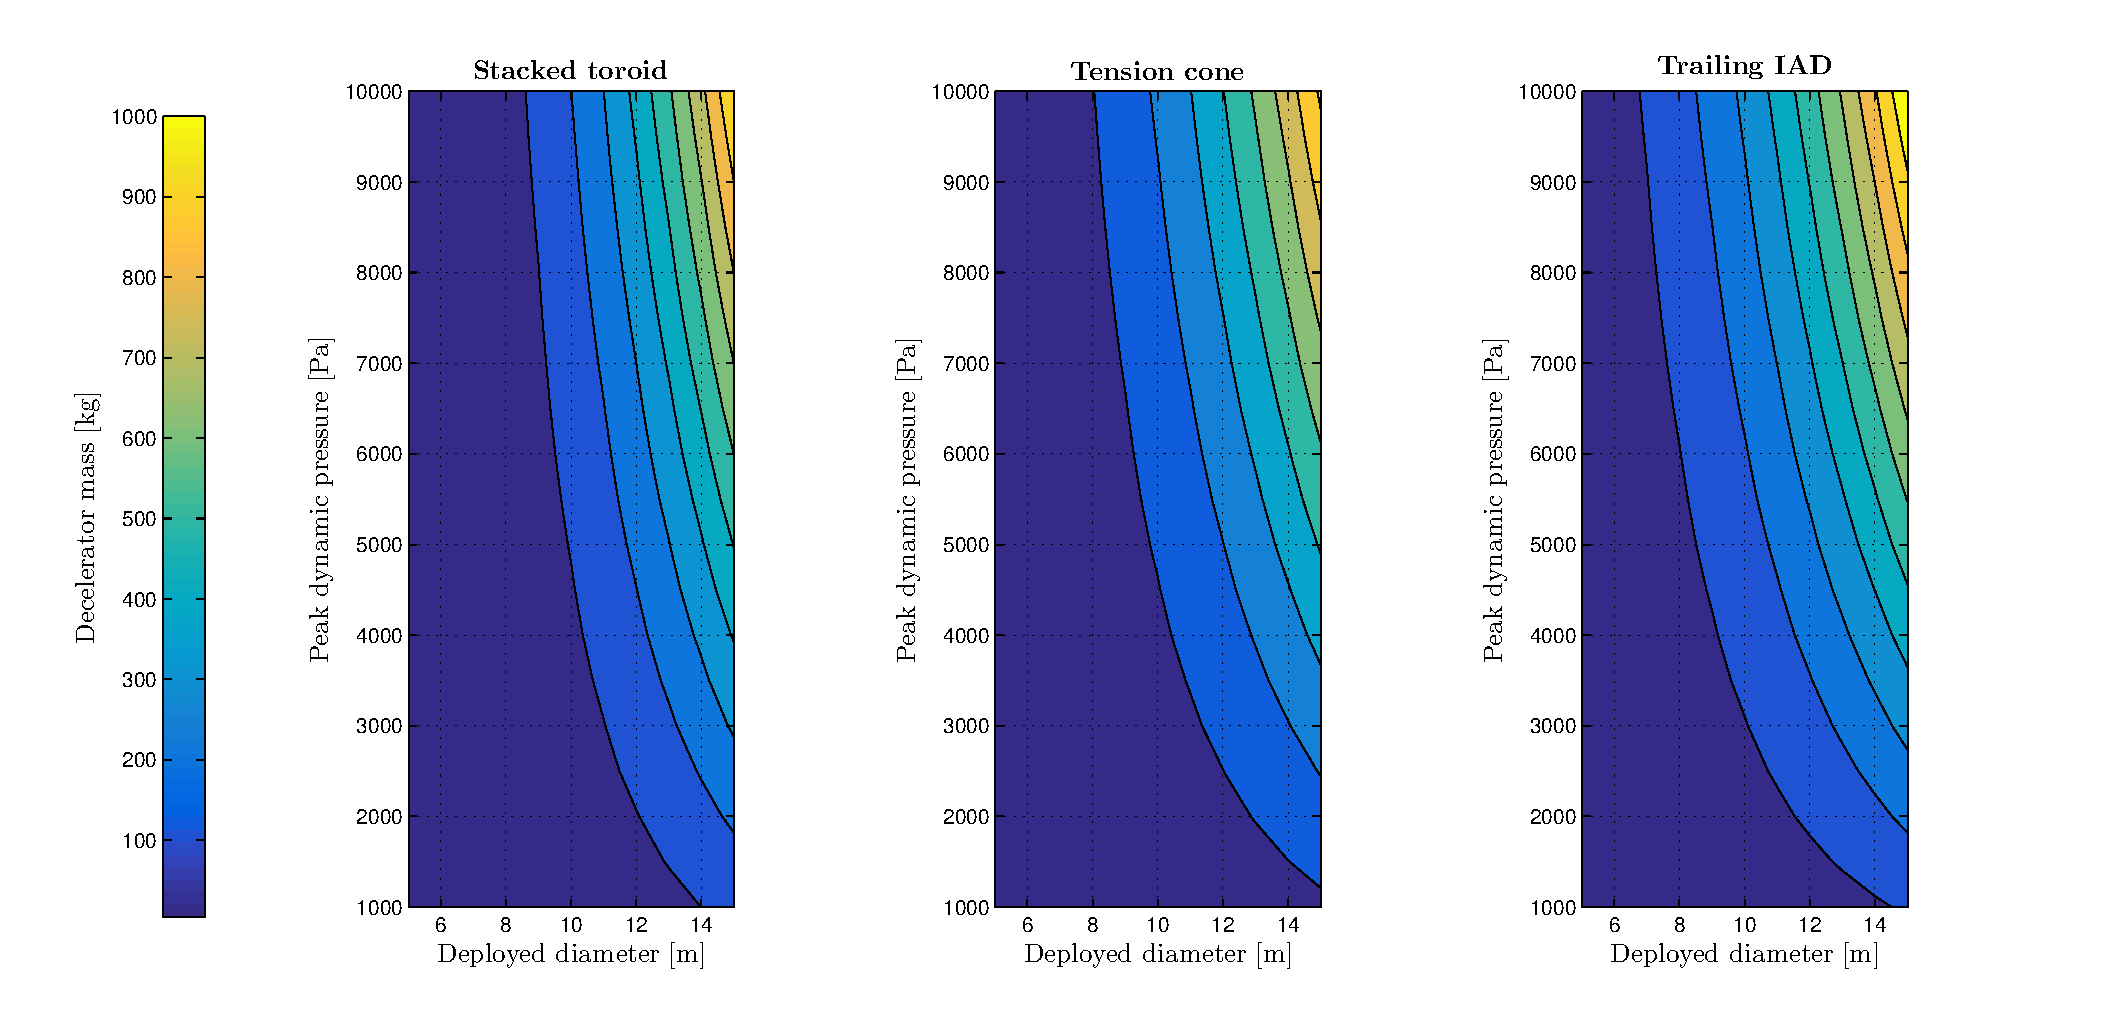
\includegraphics[width = 1.2\textwidth]{Figure/mass_dia_qmax.eps}
\caption{Decelerator structural mass as a function of peak dynamic pressure and deployed diameter for stacked toroid, tension cone and trailing ballute concepts for \gls{sym:CD} = 1.5 [-]}
\label{fig:mass_dia_qmax}
\end{figure}

\begin{figure}[H]
\centering
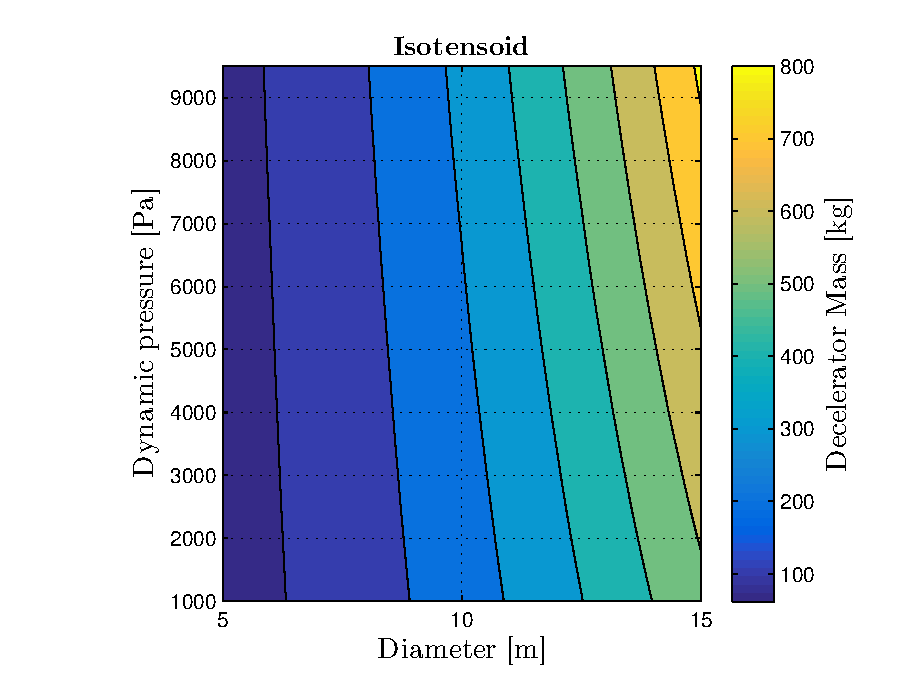
\includegraphics[width = 0.55\textwidth]{Figure/ISO_comp.eps}
\caption{Decelerator structural mass as a function of peak dynamic pressure and deployed diameter for the isotensoid concept for \gls{sym:CD} = 1.5 [-]}
\label{fig:ISO_comp}
\end{figure}

%Fig.\ref{fig:mass_dia} gives the total structural decelerator mass Figure \ref{fig:mass_dia} was made with a peak dynamic pressure of $\gls{sym:q}=3000$ [$Pa$], a drag coefficient $\gls{sym:CD}=1.5$ [$-$] and Vectran for inflatable decelerator material.

Figures \ref{fig:mass_dia_qmax} and \ref{fig:ISO_comp} show the total structural decelerator mass for the stacked toroid, tension cone, trailing ballute and isotensoid configurations, for a drag coefficient of 1.5 [-]. An increase or decrease in drag coefficient has, qualitatively, the same effect as an increase or decrease in dynamic pressure respectively. Total mass has been plotted as a function of peak dynamic pressure on one hand to display its dependence on loading conditions, as the peak dynamic pressure can be treated as a surrogate for the maximum structural loads, and as a function of deployed diameter on the other hand, since this is the primary design parameter used in the orbital analysis. 
%As both factors are held variable before concept selection after trade-off, concepts are evaluated for their mass performance over the ranges considered. 
%Peak dynamic pressures from 1000 to 10000 [Pa] are deemed representative, based on reference missions and the orbital analysis tool; diameter is constrained to 12 [m] but evaluated up to 15 [m] for the sake of completeness. 

Fig.\ref{fig:mass_dia} presents the decelerator structural mass for all four concepts in one plot, for a peak dynamic pressure of 3000 [Pa] and a drag coefficient of 1.5 [-], to better illustrate the mass differences between the different concepts. Similar plots at different peak dynamic pressures show the same trends, as follows from Figures \ref{fig:mass_dia_qmax} and \ref{fig:ISO_comp}, although mass differences become more pronounced as peak dynamic pressure is increased.

From Figures \ref{fig:mass_dia_qmax} and \ref{fig:ISO_comp} it can be observed that all concepts scale similarly with dynamic pressure and deployed diameter, but weight advantages feature more prominently at higher dynamic pressures and larger deployed diameters. For all dynamic pressures and diameters considered, the stacked toroid concept is the lightest. It is followed upon by the tension cone and trailing ballute concepts. The highest structural mass is prominently achieved by the isotensoid configuration. The tension cone is the second-lightest concept for deployed diameters greater than 6.5 [m] and the trailing ballute for deployed diameters smaller than 6.5 [m]. Notable in Fig.\ref{fig:mass_dia} is that the isotensoid configuration features a significantly higher mass than the other three configurations for a deployed diameter of 5 [m]. This is caused by the fact that Figures \ref{fig:mass_dia_qmax} and \ref{fig:ISO_comp} are produced for a centerbody diameter of 5 [m]. In the model implemented for stacked toroid, tension cone and trailing ballute \cite{Samareh2011} structural mass estimation, a dependence on both deployed and centerbody diameter is present. In this context, a deployed and centerbody diameter of 5 [m] effectively means no inflatable device is mounted, hence a zero mass. The model for the isotensoid, on the other hand, \cite{Anderson1969} does not feature any dependence on the centerbody diameter and hence the isotensoid is defined for a deployed diameter of 5 [m].

It should be noted that this comparison is based on equal drag coefficients, deployed diameter and peak dynamic pressure for all four concepts. In reality, however, each concept features a different trajectory and optimal aerodynamic shape. As such, the points in Figures \ref{fig:mass_dia_qmax} and \ref{fig:ISO_comp} at which mass is evaluated are not necessarily the same for all concepts. By a lack of detailed analysis in the difference in orbit and aerodynamic characteristics of each of the concepts within the limited timeframe, this is not taken into account. The mass comparison is therefore, however, only qualitative of nature. Mass differences between the concepts are, however, highly pronounced - at least 20 $\%$ for peak dynamic pressures higher than 2000 [Pa], deemed a reasonable lower limit based on the trajectory analysis, and a deployed diameter larger than 10 [m] - such that the comparison is deemed of adequate quality for use in the trade-off.

%Fig.\ref{fig:mass_dia} serves to show how each different configurations mass scales with varying deployed diameter. It can be noted that the isotensoid configuration has a relatively, compared to the other inflatable concepts, high mass at the base diameter of five meters. 

%This can be attributed to the fact that the isotensoid configuration features no deployed diameter. Different from the other inflatable concepts described by the model of Samareh in which the undeployed diameter has direct links the the mass of for example the gas system. The isotensoid configuration, among featuring no pressurised gas inflation system but rather ram-air, has no such diameter defined. The isotensoid is a single all compassing inflatable covering the whole payload. 

%Although plotted for set values of the drag coefficient, peak dynamic pressure and further configuration parameters important remarks with respect to the isotensoid design can already be made. If looking solely of the structural mass performance of the decelerator concepts a isotensoid configuration is the least preferable. This is further reinforced by the sensitivity analysis of section \ref{sec:strucsens} in which configuration sensitivity is further considered. 

\begin{figure}[H]
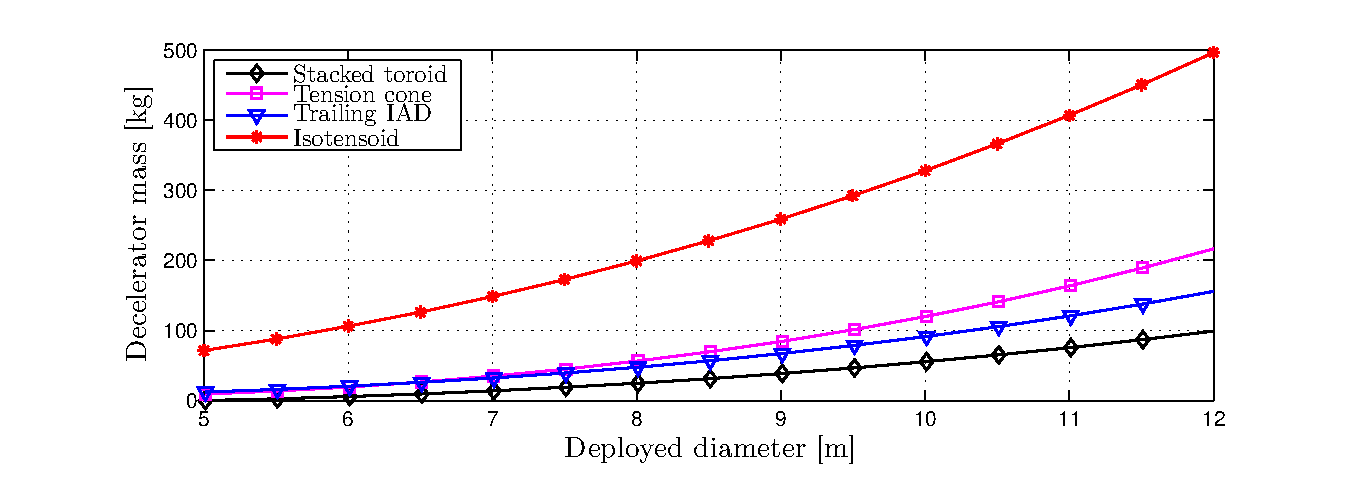
\includegraphics[width = 1.0\textwidth]{Figure/mass_dia_2300qmax.eps}
\caption{Decelerator mass versus deployed diameter for all the inflatable configurations, for a peak dynamic pressure of 2400 [Pa] and \gls{sym:CD} = 1.5 [-]}
\label{fig:mass_dia}
\end{figure}

Evaluating the decelerator mass at a peak dynamic pressure of 2400 [Pa], following from the orbit selected in Chapter \ref{ch:astrocontrol}, and a deployed diameter of 12 [m], the upper limit as dictated by requirements, yields inflatable concept mass estimations given in Table \ref{tab:strucmass}. 

\begin{table}[h]
\caption{Decelerator structural mass comparison}
\hspace{-8mm}
\begin{tabular}{|l|l|l|l|l|}
\hline
\textbf{Concept {[}-{]}}                                                                                               & Stacked toroid & Tension cone & Trailing ballute & Isotensoid \\ \hline
\textbf{Decelerator structural mass {[}kg{]}}                                                                          & 95.2             & 159          & 211              & 489        \\ \hline
\textbf{\begin{tabular}[c]{@{}l@{}}Decelerator structural mass {[}\%{]}\\     (w.r.t. lightest solution)\end{tabular}} & 100            & 168         & 221 & 516 \\ \hline
\end{tabular}
\label{tab:strucmass}
\end{table}